\documentclass[a4paper,12pt]{article}
\usepackage[utf8x]{inputenc} %fac
%\usepackage[utf8]{inputenc} %fac

\usepackage[square,sort,comma]{natbib}
%\usepackage{chapterbib}

\usepackage[francais]{babel} %FR
\usepackage[T1]{fontenc}
\usepackage{fancyhdr}

\usepackage[pdftex]{graphicx} % img
%\usepackage{wrapfig} %fac
\usepackage{float}

\usepackage{algpseudocode} %fac
\usepackage[hidelinks=true]{hyperref} %fac

\usepackage[top=3.5cm, bottom=3.5cm, left=3cm, right=3cm]{geometry} %Réduire les marges

% \usepackage{showkeys}
% \usepackage{showlabels}
\usepackage{nameref}

% Style Page
\pagestyle{fancy} % entêtes

\setlength{\headheight}{15pt}
\lhead{ \leftmark }
\rhead{ %\rightmark 
}

\sloppy % ne pas faire déborder les lignes dans la marge

%\setcounter{tocdepth}{1} %hideallsubsections

\begin{document}
  \begin{titlepage}
   \def\titletype{Cahier des charges}
   %%%%%%%%%%%%%%%%%%%%%%%%%%%%%%%%%%%%%%%%%
% University Assignment Title Page
% LaTeX Template
%
% This template has been downloaded from:
% http://www.latextemplates.com
%
% Original author:
% WikiBooks (http://en.wikibooks.org/wiki/LaTeX/Title_Creation)
%
% Instructions for using this template:
% This title page is presently capable of being compiled as is. This is not
% useful for including it in another document. To do this, you have two options:
%
% 1) Copy/paste everything between \begin{document} and \end{document}
% starting at \begin{titlepage} and paste this into another LaTeX file where you
% want your title page.
% OR
% 2) Remove everything outside the \begin{titlepage} and \end{titlepage} and
% move this file to the same directory as the LaTeX file you wish to add it to.
% Then add \input{./title_page_1.tex} to your LaTeX file where you want your
% title page.
%
%%%%%%%%%%%%%%%%%%%%%%%%%%%%%%%%%%%%%%%%%

%----------------------------------------------------------------------------------------
%       PACKAGES AND OTHER DOCUMENT CONFIGURATIONS
%----------------------------------------------------------------------------------------

\begin{titlepage}

\newcommand{\HRule}{\rule{\linewidth}{0.5mm}} % Defines a new command for the horizontal lines, change thickness here

\center % Center everything on the page

%----------------------------------------------------------------------------------------
%       HEADING SECTIONS
%----------------------------------------------------------------------------------------

\textsc{\LARGE Pierre and Marie Curie University}\\[1.5cm] % Name of your university/college
\textsc{\Large \titletype}\\[0.5cm] % Major heading such as course name
%\textsc{\large PIAD de Master1 d’Informatique en Intelligence Artificielle et Décision}\\[0.5cm] % Minor heading such as course title

%----------------------------------------------------------------------------------------
%       TITLE SECTION
%----------------------------------------------------------------------------------------

\HRule \\[0.4cm]
{ \huge \bfseries \majortitle}\\[0.4cm] % Title of your document
\HRule \\[1.5cm]


%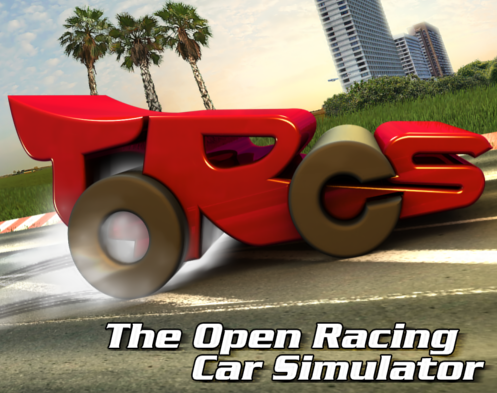
\includegraphics[height=60mm]{images/torcs.png}\\[1cm]


%----------------------------------------------------------------------------------------
%       AUTHOR SECTION
%----------------------------------------------------------------------------------------

\begin{minipage}{0.4\textwidth}
\begin{flushleft} \large
\emph{Author:}\\
Matthieu \textsc{Zimmer} % Your name
\end{flushleft}
\end{minipage}
~
\begin{minipage}{0.4\textwidth}
\begin{flushright} \large
\emph{Supervisors:} \\
Paolo \textsc{Viappiani}\\ % Supervisor's Name
Paul \textsc{Weng}\\ % Supervisor's Name
\end{flushright}
\end{minipage}\\[1cm]

\vfill

%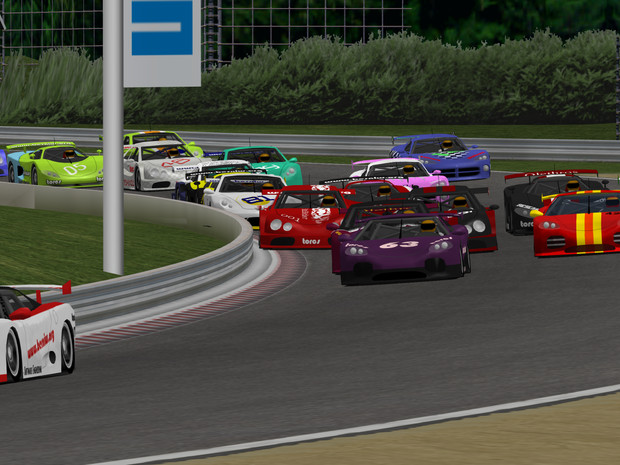
\includegraphics[height=70mm]{images/torcs.jpg}\\[1cm]

%----------------------------------------------------------------------------------------
%       DATE SECTION
%----------------------------------------------------------------------------------------

{\large \today}\\[3mm] % Date, change the \today to a set date if you want to be precise
{\large Version \docversion}\\[1.5cm]

%----------------------------------------------------------------------------------------
%       LOGO SECTION
%----------------------------------------------------------------------------------------


\includegraphics[height=13mm]{../images/logo.png} % Include a department/university logo - this will require the graphicx package

%----------------------------------------------------------------------------------------

% \vfill % Fill the rest of the page with whitespace

\end{titlepage}

  \end{titlepage}

  
  \clearpage

  \tableofcontents
  \addcontentsline{toc}{section}{Table de matière}
  
  %\vfill
  %\begin{center}
  %  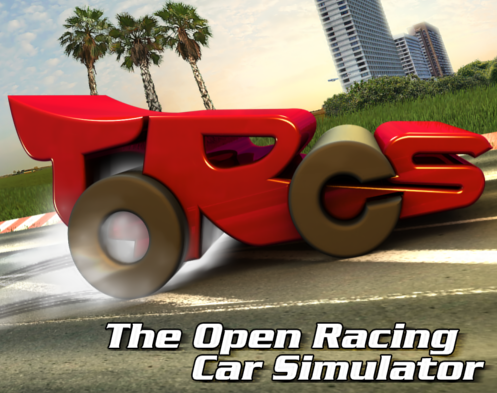
\includegraphics[height=90mm]{images/torcs.png} 
  %\end{center}

  \clearpage
  
  \renewcommand{\labelitemi}{$\bullet$}
  \renewcommand{\labelitemii}{$\circ$}
  \renewcommand{\labelitemiii}{$\diamond$}
  \renewcommand{\labelitemiv}{$\ast$}
  
  \section{Objectif du PIAD}
  \subsection{Présentation}
    Ce document représente le cahier des charges du PIAD portant sur un apprentissage semi-supervisé d'agents intelligents 
    en partant de l'\textbf{apprentissage par renforcement}.
	  
    Il s'agit de concevoir et développer un système dans lequel un agent intelligent évoluera (surveillance automatique, ...).
    Il devra être capable d'apprendre à partir de \textbf{retours limités} d'un expert humain du domaine. 
    Imaginons par exemple un agent apprenant à jouer au TETRIS : l'expert pourrait dire à l'agent où placer le 
    prochain élément ou bien si l'agent l'a bien placé. On s'attend alors à ce que cette aide diminue grandement le temps 
    d'apprentissage de l'agent.
    
  
  \subsection{Objectifs principaux}
	Nous devrons développer une \textbf{bibliothèque} indépendante du domaine dans lequel l'agent évolue. 
	Elle fournira plusieurs algorithmes de base de l'apprentissage par renforcement  (Q-Learning, SARSA, …), 
	plusieurs critères de performance, ainsi qu'une ouverture sur l'apprentissage semi-supervisé : 
	c'est à dire avec les retours de l'expert pris en compte. 
	
	Dans un premier temps, l'expert pourra simplement compenser la fonction de récompense en précisant si 
	l'agent a bien ou mal agit. Dans un second temps, si le temps le permet, l'expert pourra également agir 
	sur le choix de l'action à entreprendre lors de l'exploration de l'agent, ou encore dire à l'agent s'il 
	est temps d'exploiter ou d'explorer.
	
	Parallèlement au développement de la bibliothèque, afin d'avoir une application pratique de la théorie,
	on utilisera ces algorithmes dans le \textbf{simulateur TORCS} sur l'apprentissage automatique de la conduite de 
	voiture sur circuit. Nous modifierons également l'interface TORCS pour intégrer les retours positifs ou 
	négatifs de l'expert.

  \subsection{État de l'art}
    \paragraph{Apprentissage non supervisé} 
      L'apprentissage par renforcement fait référence à une classe de problèmes d'apprentissage automatique, 
      dont le but est d'apprendre, à partir d'expériences, ce qu'il convient de faire en différentes situations, 
      de façon à optimiser une récompense numérique au cours du temps.

      L'agent cherche, au travers d'expériences itérées, un comportement décisionnel optimal, en ce sens qu'il 
      maximise la somme des récompenses au cours du temps
      \cite{Wiki_Reinforcement_learning}.
      
      Il existe déjà de nombreux algorithmes éprouvés qu'il conviendra simplement d'implémenter
      \cite{ReinforceLearningIntro}.
  
    \vfill
    \paragraph{Apprentissage semi-supervisé} 
      Le domaine est déjà assez développé avec plusieurs algorithmes existants
      \cite{Wiki_SemiSupervised}.
      
      Pour ce qui est de l'apprentissage semi-supervisé par renforcement, il existe déjà aussi quelques articles.
  
    \paragraph{TORCS : The Open Racing Car Simulator} C'est un simulateur de course de voiture multi plate-forme.
    Il peut être utilisé comme un jeu de voiture ordinaire, ou comme plateforme de recherche en intelligence artificielle 
    car il permet de définir facilement des robots qui conduiront les voitures. 
    Son code source est sous licence GPL
    \cite{TORCS}.
    
      \begin{center}
    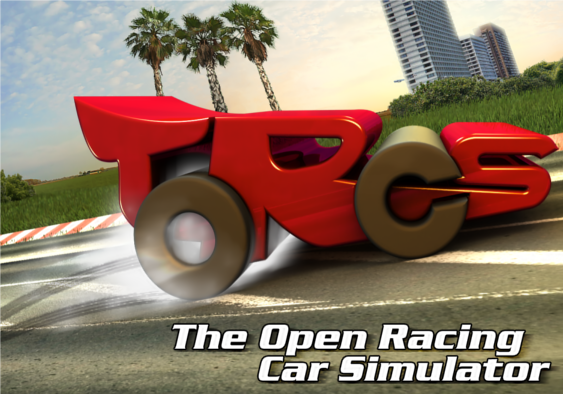
\includegraphics[height=70mm]{../images/torcs.png} 
  \end{center}
  

  \subsection{Contraintes techniques}
  
  \begin{itemize}
   \item Environnement de développement :
   \begin{itemize}
    \item Plate-forme : PC
    \item OS : Linux
    \item Langage : C++, C
    \item Outils : Doxygen, CodeBlocks, GCC, KDevelop, Cmake, Make
    \item Simulateur : TORCS
    \item Bibliothèques : Dépendances de TORCS
   \end{itemize}
   \item Contraintes matérielles requises pour faire fonctionner le système :
   \begin{itemize}
    \item 1GHz CPU
    \item 512MB RAM
    \item OpenGL 1.3 compatible graphics card with 64 MB RAM
   \end{itemize}
   \item Contraintes matérielles : toutes les fonctionnalités du système doivent pouvoir fonctionner sans 
   ralentissement dans un ordinateur de dernière génération :
   \begin{itemize}
    \item Quad Core CPU
    \item 8 GB RAM
   \end{itemize}
  \end{itemize}
  
  \vfill

  \newpage 
  \section{Description de la solution demandée}
	De nombreux termes et concepts utilisés dans cette section se réfèrent au document : \cite{PDMIA}. 
	Il est necessaire d'être familier avec les bases du \textbf{processus de décision markovien} (MDP) et de celles 
	de l'apprentissage par renforcement pour comprendre ce qui suit.
	\subsection{Fonctionnalités de la bibliothèque}
		\paragraph{Algorithmes} La bibliothèque sera composée de 2 algorithmes génériques, basés sur le critère 
		de performance $\gamma$-pondéré à horizon infini : 
		  \begin{itemize}
			  \item Q-learning
			  \item Sarsa
		  \end{itemize}
		 Ils pourront être utilisés dans n'importe quel domaine d'application.
		  
		\paragraph{Fonction de récompenses - semi supervisée} Il sera possible d'intégrer les retours d'un 
			tuteur dans la fonction de récompense. En ajoutant/retirant une constante 
			ou en multipliant la récompense par un facteur.
		\paragraph{Approximation de fonction} Lorsqu'il y a une explosition combinatoire trop importante dans
		un domaine, la bibliothèque fournira des solutions par approximation de fonction.

	\subsection{Fonctionnalités du simulateur}
		\paragraph{Robots} Les utilisateurs pourront visualiser les robots conduirent au terme ou durant leur
		apprentissage. Il sera possible de visualiser différent algorithmes :
		    \begin{itemize}
		      \item Q-learning
		      \item Sarsa
		    \end{itemize}
		\paragraph{Mesure de performance} Différentes mesures de performance pour les agents seront disponibles
		tel que : le nombre de récompenses additionnées, la durée du temps de sortie de route, dommages perçus par  
                le véhicule 
		\paragraph{Fonction de récompenses} Il sera également possible de choisir la fonction de récompense 
		tel que le fait de rester au milieu de la route, la distance parcouru
		\paragraph{Réglage des paramètres} Les paramètres tel que le taux d'apprentissage, le réglage entre
		exploitation et exploration, le taux de discrétisation des états/actions seront modifiables.
		\paragraph{Interface retour expert} Dans le cadre de l'apprentissage semi-supervisé, l'interface de TORCS
		sera modifiée pour permettre à un tuteur de donner des retours positifs ou négatifs durant l'apprentissage
		de l'agent.
	\subsection{Contraintes de réalisation}
	  \begin{itemize}
	   \item Il est primordial que les algorithmes soient \textbf{facilement interchangeables} et \textbf{réutilisables}
	   en dehors de TORCS : il doit donc y avoir une nette distinction entre le code de la librairie et
	   l'interfacement avec TORCS.
	   \item Durant la phase de conception et de développement, les documents et le code devront être maintenus 
	   en ligne (dans une forge type github) pour mettre aux encadrants de facilement suivre l'évolution du projet.
	   \item Les fonctionnalités citées précédemment constituent le \textbf{noyau central} du projet et devront être à
	   réaliser absolument. Les fonctionnalités à venir sont facultatives et leurs réalisations dépendront de 
	   l'avancement du projet.
	  \end{itemize}
		
	\subsection{Fonctionnalités additionnelles de la bibliothèque}
	  \paragraph{Algorithmes} Un algorithme de \textbf{différence temporelle} pourra être ajouté.
	  
	  \paragraph{Fonction de récompenses - semi supervisée} L'expert pourra intégrer des feedbacks plus complexes
	  tel que la prochaine action à choisir ou le renseigner sur sa stratégie exploration/exploitation.
	  
	\subsection{Fonctionnalités additionnelles du simulateur}
	  \paragraph{Robots} L'algorithme de \textbf{différence temporelle} sera également disponible.
	  \paragraph{Interface retour expert} L'interface de TORCS sera modifiée avec toute une partie indépendante
	  pour permettre au tuteur de voir les détails de l'exécution de l'algorithme et intégrer des retours plus 
	  complexes (choix d'action, stratégie exploitation/exploration).
	  \paragraph{Course multijoueur} Il sera également possible d'aborder les courses à plusieurs conducteurs. En 
	  ce sens, on pourra alors fournir de nouvelles fonctions de récompense et mesures de performance
	  tel que la position dans la course.
	  
  
  \newpage
  \section{Composition du délivrable}
  
  Dans le cadre de la réalisation du projet, nous nous engageons à livrer les produits suivants : 
  \begin{itemize}
   \item La bibliothèque implantant toutes les fonctionnalités prévues
   \item Le simulateur modifié de TORCS avec :
    \begin{itemize}
     \item Les robots implémentant les algorithmes d'apprentissage
     \item Les modifications de l'interface pour intégrer les retours de l'expert 
    \end{itemize}
   \item Le code source entièrement commentés (hormis celui de TORCS que nous n'aurons pas modifié)
   \item Un ensemble de script facilitant la compilation et l'installation
   \item La documentation complète du projet à savoir :
    \begin{itemize}
      \item Cahier des charges
      \item Plan de développement
      \item Analyse et conception
      \item Manuel d’installation
      \item Manuel de l’utilisateur
      \item Manuel du programmeur
      \item Rapport d'expériences décrivant les résultats complets en fonction des différentes routes, algorithmes et critères
      \item Rapport final
    \end{itemize}
  \end{itemize}
  
  
  
\newpage
\addcontentsline{toc}{section}{Références}
\bibliographystyle{../dependance/apalike}
\bibliography{../dependance/biblio}

\end{document}



